\documentclass{standalone}
\usepackage[T1]{fontenc}
\usepackage[utf8]{inputenc}
\usepackage{pgf,tikz}
\usepackage{setspace}
\usepackage{pgfplots}
\pgfplotsset{compat=1.13}
\usepackage{romannum}

\usepgfplotslibrary{groupplots}

\begin{document}



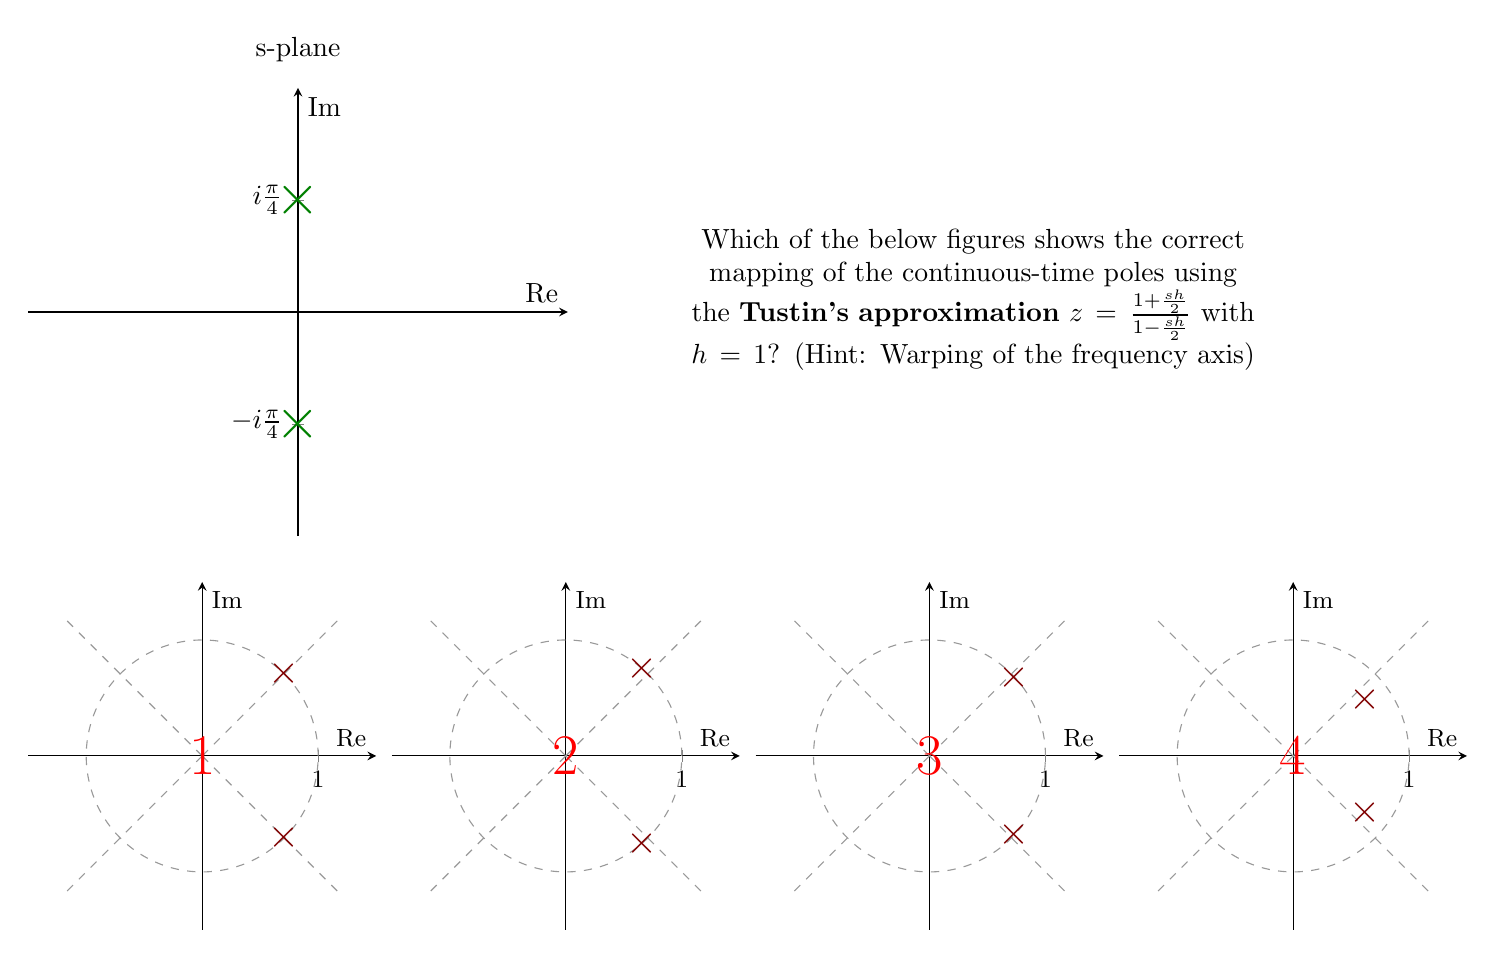
\begin{tikzpicture}

\begin{axis}[
  yshift=5cm,
  axis lines=middle, 
  xmin=-1, xmax=1,
  ymin=-2, ymax=2,
  xlabel={Re},
  ylabel={Im},
  xtick=\empty,
  ytick = {-1, 1},
  yticklabels = {$-i\frac{\pi}{4}$, $i\frac{\pi}{4}$},
  title={s-plane}
]
\node[black!50!green!100] at (axis cs: 0, -1) {\huge $\times$};
\node[black!50!green!100] at (axis cs: 0, 1) {\huge $\times$};
\end{axis}

\node[align=center, text width=8cm] at (12,8) {Which of the below figures shows the correct mapping of the continuous-time poles using the \textbf{Tustin's approximation} $z = \frac{1+\frac{sh}{2}}{1-\frac{sh}{2}}$ with $h=1$? (Hint: Warping of the frequency axis)};

\pgfplotsset{unitcircle/.style={black!40, thin, dashed, no marks}}

\pgfmathsetmacro{\ww}{pi/4}
\pgfmathsetmacro{\hh}{1}

\pgfmathsetmacro{\xone}{cos(deg(\ww*\hh))}
\pgfmathsetmacro{\yone}{sin(deg(\ww*\hh))}

\pgfmathsetmacro{\xtwo}{cos(deg(\ww*\hh)+4)}
\pgfmathsetmacro{\ytwo}{sin(deg(\ww*\hh)+4)}



\pgfmathsetmacro{\threeden}{1  + pow(\ww*\hh/2, 2)}
\pgfmathsetmacro{\xthree}{(1-pow(\ww*\hh/2, 2))/\threeden}
\pgfmathsetmacro{\ythree}{(\ww*\hh)/\threeden}


\pgfmathsetmacro{\cmagn}{1 + pow(\ww*\hh, 2)}
\pgfmathsetmacro{\xfour}{1/\cmagn}
\pgfmathsetmacro{\yfour}{\ww*\hh/\cmagn}

\def\axlim{1.5}
\begin{groupplot}[
  group style={group size=4 by 1, horizontal sep=2mm,},
  height=6cm,width=6cm,
  /tikz/font=\small,
  xtick={1},
  ytick=\empty,
  xlabel={Re},
  ylabel={Im},
  xmin=-\axlim,
  xmax=\axlim,
  ymin=-\axlim,
  ymax=\axlim,
  axis lines=middle,
  ]

  \nextgroupplot
    \addplot[unitcircle, domain=0:360, samples=361, variable=x] ( {cos(x)}, {sin(x)} );
    \addplot[unitcircle,] coordinates { (0,0) (0.8*\axlim, 0.8*\axlim) };
    \addplot[unitcircle,] coordinates { (0,0) (-0.8*\axlim, 0.8*\axlim) };
    \addplot[unitcircle,] coordinates { (0,0) (-0.8*\axlim, -0.8*\axlim) };
    \addplot[unitcircle,] coordinates { (0,0) (0.8*\axlim, -0.8*\axlim) };

    \node[black!50!red!100] at (axis cs: \xone, \yone) {\Large $\times$};
    \node[black!50!red!100] at (axis cs: \xone, -\yone) {\Large $\times$};


  \nextgroupplot
    \addplot[unitcircle, domain=0:360, samples=361, variable=x] ( {cos(x)}, {sin(x)} );
    \addplot[unitcircle,] coordinates { (0,0) (0.8*\axlim, 0.8*\axlim) };
    \addplot[unitcircle,] coordinates { (0,0) (-0.8*\axlim, 0.8*\axlim) };
    \addplot[unitcircle,] coordinates { (0,0) (-0.8*\axlim, -0.8*\axlim) };
    \addplot[unitcircle,] coordinates { (0,0) (0.8*\axlim, -0.8*\axlim) };
    \node[black!50!red!100] at (axis cs: \xtwo, \ytwo) {\Large $\times$};
    \node[black!50!red!100] at (axis cs: \xtwo, -\ytwo) {\Large $\times$};

  \nextgroupplot
    \addplot[unitcircle, domain=0:360, samples=361, variable=x] ( {cos(x)}, {sin(x)} );
    \addplot[unitcircle,] coordinates { (0,0) (0.8*\axlim, 0.8*\axlim) };
    \addplot[unitcircle,] coordinates { (0,0) (-0.8*\axlim, 0.8*\axlim) };
    \addplot[unitcircle,] coordinates { (0,0) (-0.8*\axlim, -0.8*\axlim) };
    \addplot[unitcircle,] coordinates { (0,0) (0.8*\axlim, -0.8*\axlim) };
    \node[black!50!red!100] at (axis cs: \xthree, \ythree) {\Large $\times$};
    \node[black!50!red!100] at (axis cs: \xthree, -\ythree) {\Large $\times$};

  \nextgroupplot
    \addplot[unitcircle, domain=0:360, samples=361, variable=x] ( {cos(x)}, {sin(x)} );
    \addplot[unitcircle,] coordinates { (0,0) (0.8*\axlim, 0.8*\axlim) };
    \addplot[unitcircle,] coordinates { (0,0) (-0.8*\axlim, 0.8*\axlim) };
    \addplot[unitcircle,] coordinates { (0,0) (-0.8*\axlim, -0.8*\axlim) };
    \addplot[unitcircle,] coordinates { (0,0) (0.8*\axlim, -0.8*\axlim) };
    \node[black!50!red!100] at (axis cs: \xfour, \yfour) {\Large $\times$};
    \node[black!50!red!100] at (axis cs: \xfour, -\yfour) {\Large $\times$};


  \end{groupplot}

  %\node[red] at (group c1r1.center) {\large \Romannum{1}};
  \node[red] at (group c1r1.center) {\huge 1};
  \node[red] at (group c2r1.center) {\huge 2};
  \node[red] at (group c3r1.center) {\huge 3};
  \node[red] at (group c4r1.center) {\huge 4};


\end{tikzpicture}
\end{document}

